\documentclass[11pt,a4paper]{article}

% Fonte em portgues brasileiro
\usepackage[brazilian]{babel}
\usepackage[utf8]{inputenc}
\usepackage[T1]{fontenc}
\usepackage{lmodern}

%%%%%%%%%%Packages opcionais%%%%%%%%%%%%%%

% Tabelas
\usepackage{booktabs}
\usepackage{multirow}
\usepackage{multicol}     

% Identação e espaçamento
\usepackage{fullpage}      % Autoscale da página
\usepackage{indentfirst}   % Identar parágrafo em cada quebra de linha

% Figuras
\usepackage{graphicx}      % Pictures
\graphicspath{{./logo/}{./figuras/}} % Pastas para procurar imagens

% URLs na bibliografia
\usepackage{url}

\begin{document}


%---------------------------------------------------
%Começo da capa
\begin{center}
\thispagestyle{empty}

\includegraphics[width=0.2\linewidth]{logo.png} \\[0.3cm]
\textsc{\LARGE University of Whatever}\\[1.5cm]

\textsc{\large A \LaTeX template}\\[0.5cm]
% Título
\hrule \vspace{0.4cm}
{ \huge \bfseries Trabalho  \\[0.4cm] }
\hrule \vspace{1.5cm}
\vspace{1cm} % Valor opcional, pode ser definido para alterar a altura dos nomes na página

% Autores e professor
\begin{minipage}{0.5\textwidth}
\begin{flushleft} \large
% Nomes dos alunos
\emph{Alunos:}\\
Fulano \\
Ciclano
\end{flushleft}
\end{minipage}
\begin{minipage}{0.4\textwidth}
\begin{flushright} \large
\emph{Professor:} \\
Beltrano
\end{flushright}
\end{minipage}

\vfill

% Fim da capa
{\large Cidade \\[0.4cm] Outubro de 2015}

\end{center}
% Fim da capa
%---------------------------------------------------



%---------------------------------------------------
%Começo do Sumário
\newpage
% Gerar sumário. É necessário mais de uma compilação para ser gerado completamente.
\tableofcontents
\newpage
% Fim do sumário
%---------------------------------------------------


\section{Introdução}

Esse é um arquivo base de introdução ao LaTeX. Alguns exemplos podem ser encontrados nesse texto, como por exemplo:
\\

\textbf{Esse texto está em negrito.}

\textit{Esse texto está em itálico.}

``Este texto está entre aspas''


\section{Desenvolvimento}

\subsection{Adicionando imagens}

Imagens podem ser adicionadas usando o package \texttt{usepackage\{graphicx\}}. Assim:

\begin{figure}[!ht] % O h significa here, t top e b bottom. O LaTeX joga a imagem onde for mais conveniente
\centering
	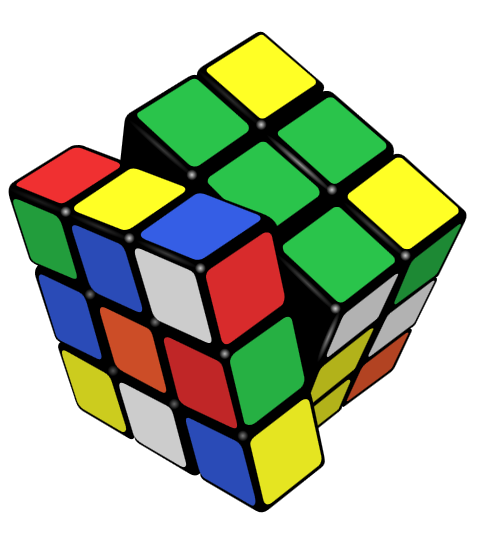
\includegraphics[width=5cm]{rubiks.png}
	\caption{Imagem Legal}
	\label{fig:cube}
\end{figure}

Podemos citar a Figura com Figura \ref{fig:cube}.

Podemos adicionar duas Figuras lado a lado utilizando o ambiente \texttt{minipage} dentro do ambiente \texttt{figure}

\begin{figure}[!h]
  \centering
  \begin{minipage}[b]{0.4\textwidth}
  	\centering
    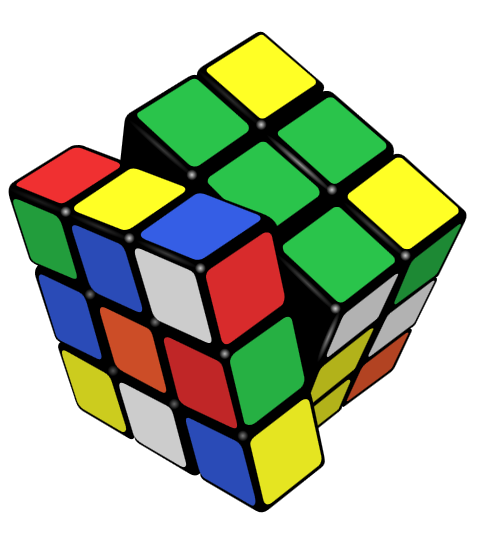
\includegraphics[width=.5\textwidth]{rubiks.png}   % Figura 1
    \caption{Uma figura}
  \end{minipage}
  \begin{minipage}[b]{0.4\textwidth}
  	\centering
    
\includegraphics[width=.5\textwidth]{logo.png}     % Figura 2
    \caption{Outra figura}
  \end{minipage}
\end{figure}


\subsection{Adicionando tabelas}

Para adicionar utilizaremos o ambiente \texttt{table}. Observe a Tabela \ref{tab:tabela}.

\begin{table}[!h]
\centering
\begin{tabular}{c|c|c}   % Tabela com três elementos de largura centralizado. Utilize l para left e r para right
% Utilize as 'rules' para traços na tabela
\toprule
Potência   &    Número  & Primos menores que número  \\  \midrule
1  &    10      &   4                        \\
2  &	100 	&   25 	                     \\
3  &	1,000   &	168 	                 \\
4  &	10,000  &	1,229 	                 \\
5  &	100,000 &	9,592 	                 \\
6  &	1,000,000   & 	78,498 	             \\
7  &	10,000,000  &	664,579 	         \\
8  &	100,000,000 &	5,761,455 	         \\
9  &    1,000,000,000  &	50,847,534 	     \\
10 &	10,000,000,000 &	455,052,511      \\   \toprule \bottomrule
\end{tabular}
\caption{Distribuição de Primos $\pi(x)$} \label{tab:tabela}
\end{table}


\subsection{Equações}

\subsubsection{Mathmode}

Para utilizar o Mathmode cerque a expressão por cifrões. Por exemplo \verb!$E = mc^2$!  produzirá $E = mc^2$. Para equações mais complexas que ocupem a própria linha utilize um cifrão duplo. \verb!$$E_r = \sqrt{ (m_0 c^2)^2 + (pc)^2 }$$! produzirá:

$$E_r = \sqrt{ (m_0 c^2)^2 + (pc)^2 }$$

\subsection{Ambiente \texttt{Equation}}

Pode-se utilizar o comando \texttt{Equation} para equações numeradas:

\begin{equation} \label{equ:equação}
\Delta t' = \gamma \, \Delta t = \frac{\Delta t}{\sqrt{1-\frac{v^2}{c^2}}}
\end{equation}

A Equação \ref{equ:equação} representa a dilatação temporal segundo a Teoria da Relatividade.

\subsection{Citações}

Para dar nome citável às imagens e tabelas foi utilizado o comando \verb!\label{•}!. Para citar, é utilizado \verb!\ref{•}!. Para citar bibliografia, adicione a entrada no arquivo \texttt{bibliography.bib} e utilize \verb!\cite{•}!.

Essa é uma citação exemplo e fictícia a um livro \cite{SIAM}. Essa é outra citação fictícia a uma página web \cite{wiki}.

Para mais informações acesse a página sobre referências em Wikibooks \cite{latex}.

\newpage
% Gerar bibliografia
% É necessário a compilação PdfLatex > BibTex > PdfLatex > PdfLatex, já que o arquivo bibliography é compilado separadamente.
\bibliographystyle{ieeetr}
\bibliography{bibliography}


\end{document}
